\documentclass[a4paper,11pt]{article}
\usepackage{amsmath,amsthm,amsfonts,amssymb,amscd,amstext,vmargin,graphics,graphicx,tabularx,multicol} 
\usepackage[francais]{babel}
\usepackage[utf8]{inputenc}  
\usepackage[T1]{fontenc} 
\usepackage{pstricks-add,tikz,tkz-tab,variations}
\usepackage[autolanguage,np]{numprint} 
\usepackage{color}

\setmarginsrb{1.5cm}{0.5cm}{1cm}{0.5cm}{0cm}{0cm}{0cm}{0cm} %Gauche, haut, droite, haut
\newcounter{numexo}
\newcommand{\exo}[1]{\stepcounter{numexo}\noindent{\bf Exercice~\thenumexo} : \marginpar{\hfill /#1}}
\reversemarginpar


\newcounter{enumtabi}
\newcounter{enumtaba}
\newcommand{\q}{\stepcounter{enumtabi} \theenumtabi.  }
\newcommand{\qa}{\stepcounter{enumtaba} (\alph{enumtaba}) }
\newcommand{\initq}{\setcounter{enumtabi}{0}}
\newcommand{\initqa}{\setcounter{enumtaba}{0}}

\newcommand{\be}{\begin{enumerate}}
\newcommand{\ee}{\end{enumerate}}
\newcommand{\bi}{\begin{itemize}}
\newcommand{\ei}{\end{itemize}}
\newcommand{\bp}{\begin{pspicture*}}
\newcommand{\ep}{\end{pspicture*}}
\newcommand{\bt}{\begin{tabular}}
\newcommand{\et}{\end{tabular}}
\renewcommand{\tabularxcolumn}[1]{>{\centering}m{#1}} %(colonne m{} centrée, au lieu de p par défault) 
\newcommand{\tnl}{\tabularnewline}

\newcommand{\bmul}[1]{\begin{multicols}{#1}}
\newcommand{\emul}{\end{multicols}}

\newcommand{\trait}{\noindent \rule{\linewidth}{0.2mm}}
\newcommand{\hs}[1]{\hspace{#1}}
\newcommand{\vs}[1]{\vspace{#1}}

\newcommand{\N}{\mathbb{N}}
\newcommand{\Z}{\mathbb{Z}}
\newcommand{\R}{\mathbb{R}}
\newcommand{\C}{\mathbb{C}}
\newcommand{\Dcal}{\mathcal{D}}
\newcommand{\Ccal}{\mathcal{C}}
\newcommand{\mc}{\mathcal}

\newcommand{\vect}[1]{\overrightarrow{#1}}
\newcommand{\ds}{\displaystyle}
\newcommand{\eq}{\quad \Leftrightarrow \quad}
\newcommand{\vecti}{\vec{\imath}}
\newcommand{\vectj}{\vec{\jmath}}
\newcommand{\Oij}{(O;\vec{\imath}, \vec{\jmath})}
\newcommand{\OIJ}{(O;I,J)}


\newcommand{\reponse}[1][1]{%
\multido{}{#1}{\makebox[\linewidth]{\rule[0pt]{0pt}{20pt}\dotfill}
}}

\newcommand{\titre}[5] 
% #1: titre #2: haut gauche #3: bas gauche #4: haut droite #5: bas droite
{
\noindent #2 \hfill #4 \\
#3 \hfill #5

\vspace{-1.6cm}

\begin{center}\rule{6cm}{0.5mm}\end{center}
\vspace{0.2cm}
\begin{center}{\large{\textbf{#1}}}\end{center}
\begin{center}\rule{6cm}{0.5mm}\end{center}
}



\begin{document}
\pagestyle{empty}
\titre{Contrôle sur les 3 premiers chapitres }{Nom :}{Prénom :}{Classe}{Date}


\exo{3} Calculer les expressions suivantes et donner la réponse sous la forme d'une fraction irréductible :\\

$P = \dfrac{3}{5} \times \dfrac{10}{7} - \dfrac{23}{7} \div \dfrac{1}{7}$ \hspace*{0.3cm} et\hspace*{0.3cm} $ T = \dfrac{\dfrac{1}{4} + 3}{\dfrac{11}{5}-\dfrac{13}{5}}$  \\

\exo{6}

On considère la figure ci-dessous sur laquelle (ED)$\slash \slash$(BC) et AB = 7,5 ; BC = 9 ; AC = 6 : AD = 4 ; AG = 10 et AF = 8.


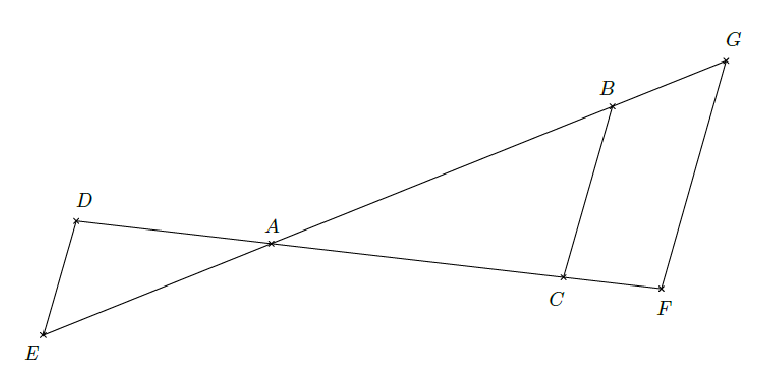
\includegraphics[scale=1]{thales1.eps} \\



\q Calculer AE et ED.\\

\q Prouver que (BC)$\slash \slash$(GF).\\


\exo{3}

\noindent Dans les marais salants, le sel récolté est stocké sur une surface plane.\\
On admet qu'un tas de sel a toujours la forme d'un cône de révolution.\\
Pascal souhaite déterminer la hauteur d'un cône de sel de diamètre 5 mètres. Il possède un bâton de longueur 1 mètre. Il effectue des mesures et réalise les deux schémas ci-dessous.\\


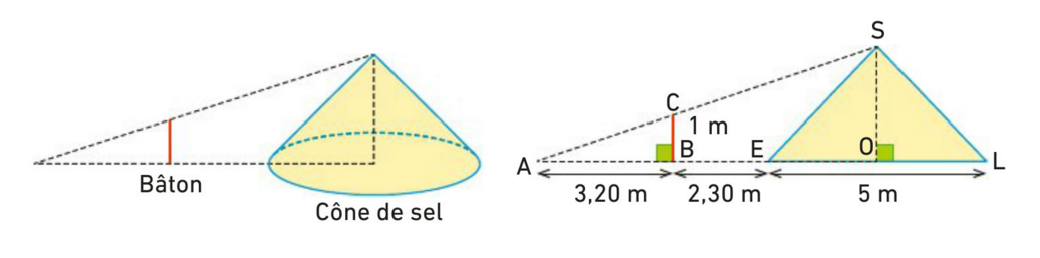
\includegraphics[scale=1]{thales2.eps} 


\initq \q Démontrer que la hauteur de ce cône de sel est égale à 2,5 mètres\\



\exo{2,5}

\initq \q Donner tous les diviseurs des nombres entiers suivants : 99; 77 000.\\

\q Parmi les six nombres suivants, quels sont ceux qui sont premiers? (\textbf{Justifier votre réponse}.)\\
1 ; 41 ; 51 ; 61 ; 71 et 81.\\

\newpage

\exo{3}

Soit $A= 140 $, $ B = 2 \times 3 \times 11$ et $C= 11 \times 13$\\

\initq \q Décomposer A en produit de facteurs premiers.\\

\q La fraction $\dfrac{A}{B}$ est-elle irréductible ? (\textbf{Justifier votre réponse}.)\\

\q Même question pour $\dfrac{A}{C}$.(\textbf{Justifier votre réponse}.)\\

\exo{2,5} Un confiseur dispose de 966 bonbons aux fruits et 690 caramels. Il souhaite faire des petits paquets tous identiques, en utilisant tous les bonbons et caramels.\\

\initq \q Le confiseur peut-il faire 115 paquets?(\textbf{Justifier votre réponse}.)

\q Quel est le nombre maximal de paquets que le confiseur peut-il réaliser ? Quelle est alors la composition de chaque paquet ?(\textbf{Justifier votre réponse à l'aide d'un calcul de PGCD}.)\\

\exo{Bonus}

On considère la figure ci-dessous sur laquelle:\\
AN vaut le plus grand des facteurs premiers de 33\\
$AC = \dfrac{2 ^ {3} \times 5 \times 11}{8}  $\\
AM vaut le plus grand des diviseurs de 30\\
$ AB = \dfrac{9}{3} \times \dfrac{\dfrac{1}{4} + \dfrac{12}{16}}{\dfrac{0}{3}+\dfrac{1}{10}}$  \\

MN est le PGCD de 36 et de 28

%AN = 11
%AC = 55
%MN = 6
%BC = 30
%AM = 

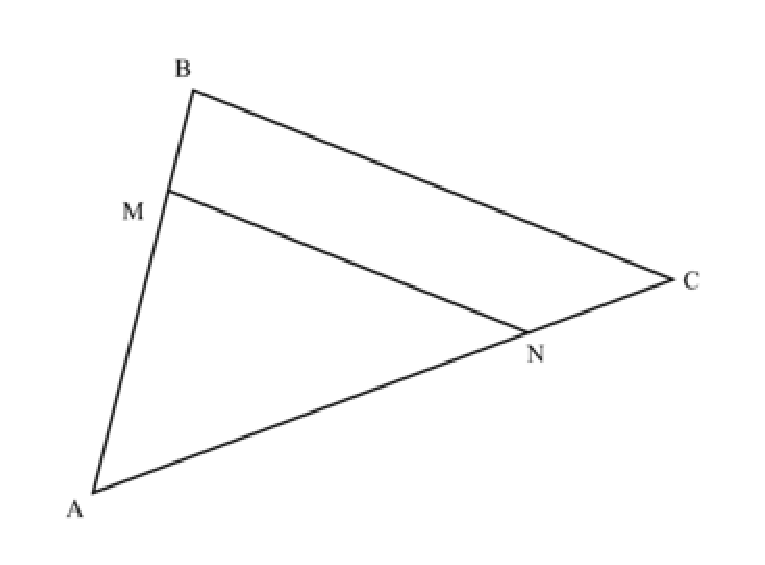
\includegraphics[scale=1]{thales3_cas_simple.eps} 

\initq \q Démontrer que les droites (MN) et (BC) sont parallèles\\

\q Calculer BC .\\


\end{document}
